\documentclass[11pt,a4paper]{report}
\usepackage[textwidth=37em,vmargin=30mm]{geometry}
\usepackage{calc,xunicode,amsmath,amssymb,paralist,enumitem,tabu,booktabs,datetime2,xeCJK,xeCJKfntef,listings}
\usepackage{tocloft,fancyhdr,tcolorbox,xcolor,graphicx,eso-pic,xltxtra,xelatexemoji}

\newcommand{\envyear}[0]{2025}
\newcommand{\envdatestr}[0]{2025-06-12}
\newcommand{\envfinaldir}[0]{webdb/2025/20250612/final}

\usepackage[hidelinks]{hyperref}
\hypersetup{
    colorlinks=false,
    pdfpagemode=FullScreen,
    pdftitle={Web Digest - \envdatestr}
}

\setlength{\cftbeforechapskip}{10pt}
\renewcommand{\cftchapfont}{\rmfamily\bfseries\large\raggedright}
\setlength{\cftbeforesecskip}{2pt}
\renewcommand{\cftsecfont}{\sffamily\small\raggedright}

\setdefaultleftmargin{2em}{2em}{1em}{1em}{1em}{1em}

\usepackage{xeCJK,xeCJKfntef}
\xeCJKsetup{PunctStyle=plain,RubberPunctSkip=false,CJKglue=\strut\hskip 0pt plus 0.1em minus 0.05em,CJKecglue=\strut\hskip 0.22em plus 0.2em}
\XeTeXlinebreaklocale "zh"
\XeTeXlinebreakskip = 0pt


\setmainfont{Brygada 1918}
\setromanfont{Brygada 1918}
\setsansfont{IBM Plex Sans}
\setmonofont{JetBrains Mono NL}
\setCJKmainfont{Noto Serif CJK SC}
\setCJKromanfont{Noto Serif CJK SC}
\setCJKsansfont{Noto Sans CJK SC}
\setCJKmonofont{Noto Sans CJK SC}

\setlength{\parindent}{0pt}
\setlength{\parskip}{8pt}
\linespread{1.15}

\lstset{
	basicstyle=\ttfamily\footnotesize,
	numbersep=5pt,
	backgroundcolor=\color{black!5},
	showspaces=false,
	showstringspaces=false,
	showtabs=false,
	tabsize=2,
	captionpos=b,
	breaklines=true,
	breakatwhitespace=true,
	breakautoindent=true,
	linewidth=\textwidth
}






\newcommand{\coverpic}[2]{
    % argv: itemurl, authorname
    Cover photo by #2~~(\href{#1}{#1})
}
\newcommand{\makeheader}[0]{
    \begin{titlepage}
        % \newgeometry{hmargin=15mm,tmargin=21mm,bmargin=12mm}
        \begin{center}
            
            \rmfamily\scshape
            \fontspec{BaskervilleF}
            \fontspec{Old Standard}
            \fontsize{59pt}{70pt}\selectfont
            WEB\hfill DIGEST
            
            \vfill
            % \vskip 30pt
            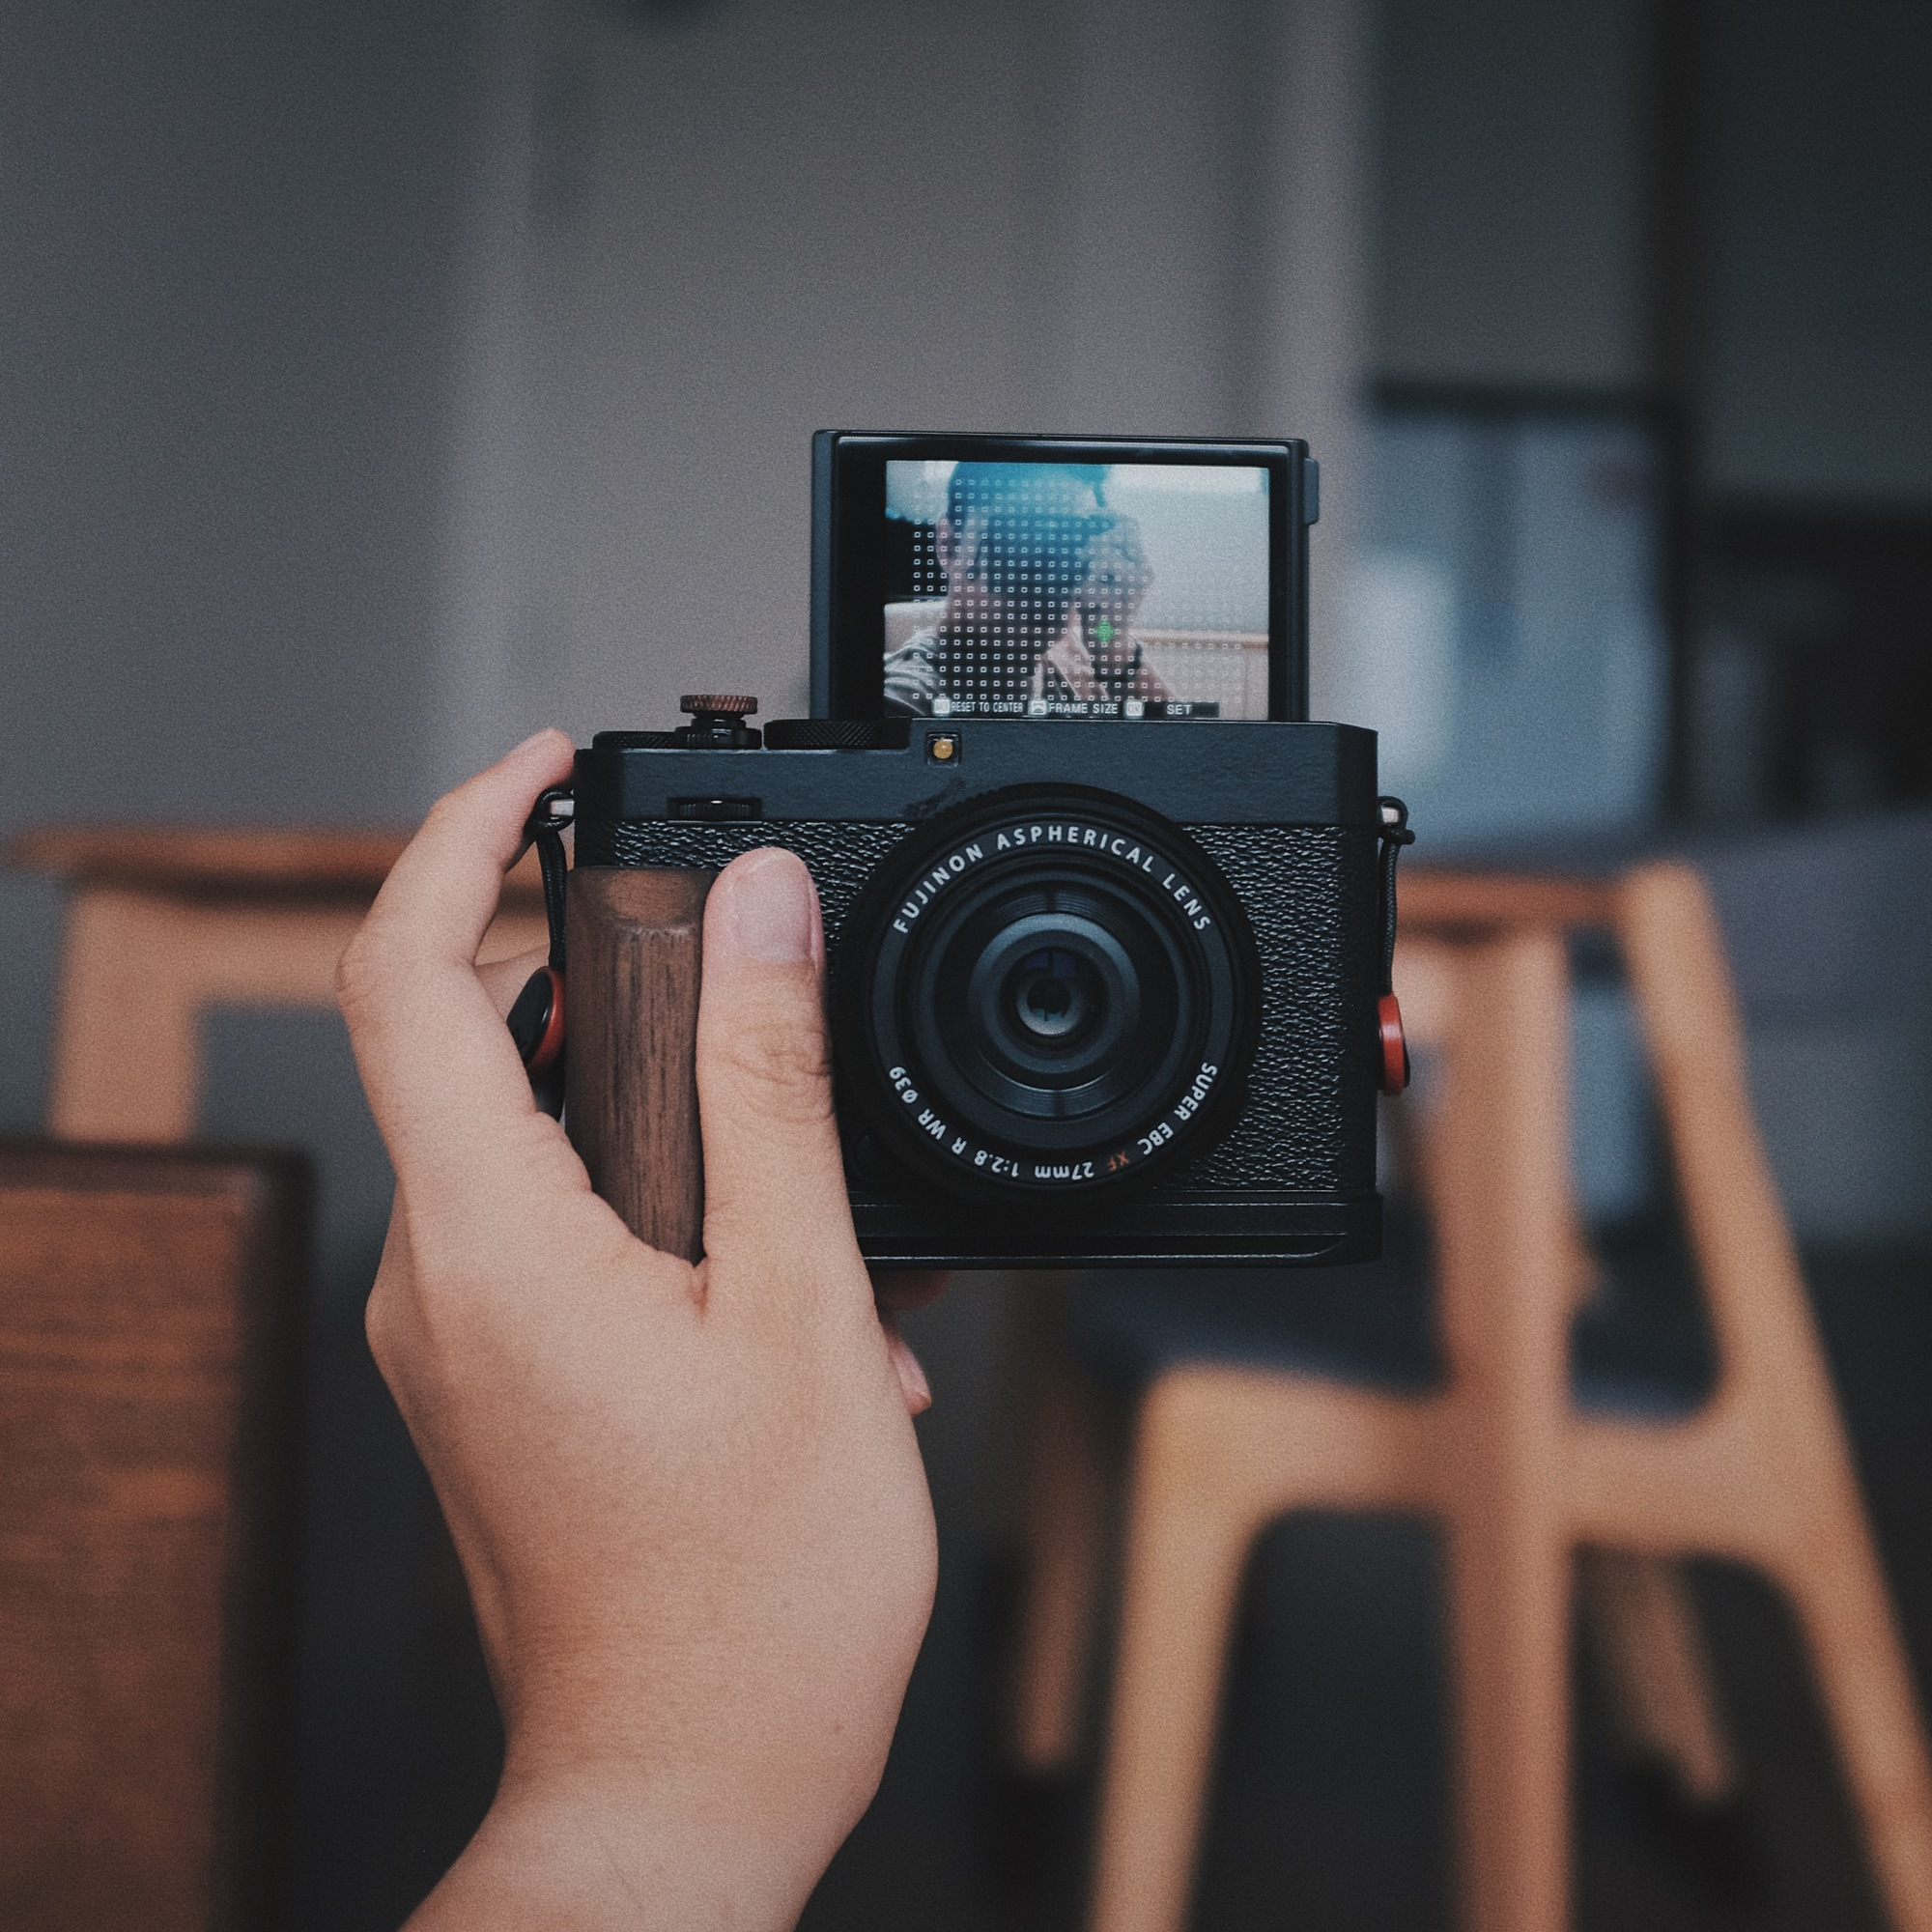
\includegraphics[width=\linewidth]{\envfinaldir/coverpic-prod.jpg}\par
            % \vskip 30pt
            \vfill

            \normalsize\rmfamily\scshape
            \copyright{} The Web Digest Project \hfill\large \envdatestr
        \end{center}
    \end{titlepage}
    % \restoregeometry
}
\newcommand{\simplehref}[1]{%
    \textcolor{blue!80!green}{\href{#1}{#1}}%
}
\renewcommand{\contentsname}{\center\Huge\sffamily\bfseries Contents\par\vskip 20pt}
\newcounter{ipartcounter}
\setcounter{ipartcounter}{0}
\newcommand{\ipart}[1]{
    % \vskip 20pt
    \clearpage
    \stepcounter{ipartcounter}
    \phantomsection
    \addcontentsline{toc}{chapter}{#1}
    % \begin{center}
    %     \Huge
    %     \sffamily\bfseries
    %     #1
    % \end{center}
    % \vskip 20pt plus 7pt
}
\newcounter{ichaptercounter}
\setcounter{ichaptercounter}{0}
\newcommand{\ichapter}[1]{
    % \vskip 20pt
    \clearpage
    \stepcounter{ichaptercounter}
    \phantomsection
    \addcontentsline{toc}{section}{\numberline{\arabic{ichaptercounter}}#1}
    \begin{center}
        \Huge
        \sffamily\bfseries
        #1
    \end{center}
    \vskip 20pt plus 7pt
}
\newcommand{\entrytitlefont}[1]{\subsection*{\raggedright\Large\sffamily\bfseries#1}}
\newcommand{\entryitemGeneric}[2]{
    % argv: title, url
    \parbox{\linewidth}{
        \entrytitlefont{#1}\par\vskip 5pt
        \footnotesize\ttfamily\mdseries
        \simplehref{#2}
    }\vskip 11pt plus 11pt minus 1pt
}
\newcommand{\entryitemGithub}[3]{
    % argv: title, url, desc
    \parbox{\linewidth}{
        \entrytitlefont{#1}\par\vskip 5pt
        \footnotesize\ttfamily\mdseries
        \simplehref{#2}\par\vskip 5pt
        \small\rmfamily\mdseries#3
    }\vskip 11pt plus 11pt minus 1pt
}
\newcommand{\entryitemAp}[3]{
    % argv: title, url, desc
    \parbox{\linewidth}{
        \entrytitlefont{#1}\par\vskip 5pt
        \footnotesize\ttfamily\mdseries
        \simplehref{#2}\par\vskip 5pt
        \small\rmfamily\mdseries#3
    }\vskip 11pt plus 11pt minus 1pt
}
\newcommand{\entryitemHackernews}[3]{
    % argv: title, hnurl, rawurl
    % \parbox{\linewidth}{
    %     \entrytitlefont{#1}\par\vskip 5pt
    %     \footnotesize\ttfamily\mdseries
    %     \simplehref{#3}\par
    %     \textcolor{black!50}{\href{#2}{#2}}
    % }\vskip 11pt plus 11pt minus 1pt
    \begin{minipage}{\linewidth}
            \entrytitlefont{#1}\par\vskip 5pt
            \footnotesize\ttfamily\mdseries
            \simplehref{#3}\par
            \textcolor{black!50}{\href{#2}{#2}}
    \end{minipage}\par\vskip 11pt plus 11pt minus 1pt
}







\begin{document}

\makeheader

\tableofcontents\clearpage




\ipart{Developers}
\ichapter{Hacker News}
\entryitemTwoLinks{Congratulations on creating the one billionth repository on GitHub}{https://news.ycombinator.com/item?id=44252076}{https://github.com/AasishPokhrel/shit/issues/1}

\entryitemTwoLinks{Chatterbox TTS}{https://news.ycombinator.com/item?id=44251411}{https://github.com/resemble-ai/chatterbox}

\entryitemTwoLinks{Research suggests Big Bang may have taken place inside a black hole}{https://news.ycombinator.com/item?id=44251047}{https://www.port.ac.uk/news-events-and-blogs/blogs/space-cosmology-and-the-universe/what-if-the-big-bang-wasnt-the-beginning-our-research-suggests-it-may-have-taken-place-inside-a-black-hole}

\entryitemTwoLinks{EchoLeak – 0-Click AI Vulnerability Enabling Data Exfiltration from 365 Copilot}{https://news.ycombinator.com/item?id=44250774}{https://www.aim.security/lp/aim-labs-echoleak-blogpost}

\entryitemTwoLinks{Show HN: Spark, An advanced 3D Gaussian Splatting renderer for Three.js}{https://news.ycombinator.com/item?id=44249565}{https://sparkjs.dev/}

\entryitemTwoLinks{Brian Wilson has died}{https://news.ycombinator.com/item?id=44249467}{https://pitchfork.com/news/the-beach-boys-brian-wilson-dies-at-82/}

\entryitemTwoLinks{Dolly Parton's Dollywood Express}{https://news.ycombinator.com/item?id=44249417}{https://thetransitguy.substack.com/p/dolly-parton-runs-a-train-busier}

\entryitemTwoLinks{Medical aid in dying, my health, and so on}{https://news.ycombinator.com/item?id=44249303}{https://blog.the-brannons.com/post/Medical-Aid-in-Dying-My-Health-and-so-on}

\entryitemTwoLinks{V-JEPA 2 world model and new benchmarks for physical reasoning}{https://news.ycombinator.com/item?id=44248165}{https://ai.meta.com/blog/v-jepa-2-world-model-benchmarks/}

\entryitemTwoLinks{AI at Amazon: A case study of brittleness}{https://news.ycombinator.com/item?id=44247998}{https://surfingcomplexity.blog/2025/06/08/ai-at-amazon-a-case-study-of-brittleness/}

\entryitemTwoLinks{Show HN: RomM – An open-source, self-hosted ROM manager and player}{https://news.ycombinator.com/item?id=44247964}{https://github.com/rommapp/romm}

\entryitemTwoLinks{Bypassing GitHub Actions policies in the dumbest way possible}{https://news.ycombinator.com/item?id=44247881}{https://blog.yossarian.net/2025/06/11/github-actions-policies-dumb-bypass}

\entryitemTwoLinks{DeskHog, an open-source developer toy}{https://news.ycombinator.com/item?id=44247501}{https://posthog.com/deskhog}

\entryitemTwoLinks{Show HN: Ikuyo a Travel Planning Web Application}{https://news.ycombinator.com/item?id=44247029}{https://ikuyo.kenrick95.org/}

\entryitemTwoLinks{Menstrual tracking app data is gold mine for advertisers that risks women safety}{https://news.ycombinator.com/item?id=44246920}{https://www.cam.ac.uk/research/news/menstrual-tracking-app-data-is-a-gold-mine-for-advertisers-that-risks-womens-safety-report}

\entryitemTwoLinks{Firefox OS's story from a Mozilla insider not working on the project (2024)}{https://news.ycombinator.com/item?id=44246518}{https://ludovic.hirlimann.net/2024/01/firefox-oss-story-from-mozila-insider.html}

\entryitemTwoLinks{Show HN: S3mini – Tiny and fast S3-compatible client, no-deps, edge-ready}{https://news.ycombinator.com/item?id=44245577}{https://github.com/good-lly/s3mini}

\entryitemTwoLinks{Left-Pad (2024)}{https://news.ycombinator.com/item?id=44245166}{https://azerkoculu.com/posts/left-pad}

\entryitemTwoLinks{Why Koreans ask what year you were born}{https://news.ycombinator.com/item?id=44244879}{https://bryanhogan.com/blog/korean-age}

\entryitemTwoLinks{It's the end of observability as we know it (and I feel fine)}{https://news.ycombinator.com/item?id=44243050}{https://www.honeycomb.io/blog/its-the-end-of-observability-as-we-know-it-and-i-feel-fine}


\ipart{Developers~~~~(zh-Hans)}
\ichapter{Solidot}
\entryitemGeneric{\hskip 0pt{}研究人员发现两个能完全绕过 Secure Boot 的漏洞利用,微软只给一个打上补丁}{https://www.solidot.org/story?sid=81528}

\entryitemGeneric{\hskip 0pt{}韦伯拍摄到寒冷气态巨行星的直接影像}{https://www.solidot.org/story?sid=81527}

\entryitemGeneric{\hskip 0pt{}全球盗版网站访问量继续下滑,但盗版漫画访问量在增长}{https://www.solidot.org/story?sid=81526}

\entryitemGeneric{\hskip 0pt{}今天的 AI 并没有智能}{https://www.solidot.org/story?sid=81525}

\entryitemGeneric{\hskip 0pt{}地球海洋酸化跨过``行星限度''}{https://www.solidot.org/story?sid=81524}

\entryitemGeneric{\hskip 0pt{}Google 发布 Android 16}{https://www.solidot.org/story?sid=81523}

\entryitemGeneric{\hskip 0pt{}Telegram、中间人以及 FSB}{https://www.solidot.org/story?sid=81522}

\entryitemGeneric{\hskip 0pt{}Ubuntu 25.10 的 GNOME 桌面环境停止支持 X11 }{https://www.solidot.org/story?sid=81521}

\entryitemGeneric{\hskip 0pt{}研究称鱼临死前经历数十分钟的痛苦}{https://www.solidot.org/story?sid=81520}

\entryitemGeneric{\hskip 0pt{}中国 AI 公司在高考期间短暂禁用了部分功能以防止考试作弊}{https://www.solidot.org/story?sid=81519}

\entryitemGeneric{\hskip 0pt{}欧洲需要数字主权}{https://www.solidot.org/story?sid=81518}

\entryitemGeneric{\hskip 0pt{}Mozilla 又关闭了两项服务}{https://www.solidot.org/story?sid=81517}

\entryitemGeneric{\hskip 0pt{}macOS Tahoe 将是最后一个支持英特尔处理器的 macOS 版本}{https://www.solidot.org/story?sid=81516}

\entryitemGeneric{\hskip 0pt{}按摩脸部和颈部或有助于大脑冲掉垃圾}{https://www.solidot.org/story?sid=81515}

\entryitemGeneric{\hskip 0pt{}人类昼夜节律与季节性阳光相关}{https://www.solidot.org/story?sid=81514}

\entryitemGeneric{\hskip 0pt{}拉斯维加斯的应对气候策略:种植更多树}{https://www.solidot.org/story?sid=81513}

\entryitemGeneric{\hskip 0pt{}报告称全球生育率普遍下滑}{https://www.solidot.org/story?sid=81512}

\entryitemGeneric{\hskip 0pt{}FAA 计划淘汰软盘和 Windows 95}{https://www.solidot.org/story?sid=81511}

\entryitemGeneric{\hskip 0pt{}印度 Manipur 邦实行宵禁并切断互联网访问}{https://www.solidot.org/story?sid=81509}

\entryitemGeneric{\hskip 0pt{}Linux 基金会试图和解围绕 WordPress 的纠纷}{https://www.solidot.org/story?sid=81508}\ichapter{V2EX}
\entryitemGeneric{\hskip 0pt{}[macOS] macos26 限制充电失效}{https://www.v2ex.com/t/1138036}

\entryitemGeneric{\hskip 0pt{}[宽带症候群] 工作室软路由分流}{https://www.v2ex.com/t/1138035}

\entryitemGeneric{\hskip 0pt{}[问与答] 数据库服务器被勒索了,文件被加密,求低成本解密办法}{https://www.v2ex.com/t/1138034}

\entryitemGeneric{\hskip 0pt{}[Linux] zed 这个编辑器值得关注}{https://www.v2ex.com/t/1138033}

\entryitemGeneric{\hskip 0pt{}[分享发现] 日历吗,更新了!}{https://www.v2ex.com/t/1138032}

\entryitemGeneric{\hskip 0pt{}[推广] XiaoMusic 因 alist 事件连夜发布版本 v0.3.83}{https://www.v2ex.com/t/1138030}

\entryitemGeneric{\hskip 0pt{}[程序员] 充了 Google One, Gemini 的智商依旧是所有 AI 垫底}{https://www.v2ex.com/t/1138029}

\entryitemGeneric{\hskip 0pt{}[NAS] 618 购买了绿联 4800,请教一些姿势}{https://www.v2ex.com/t/1138028}

\entryitemGeneric{\hskip 0pt{}[问与答] 目前那款指纹浏览器效果最好。}{https://www.v2ex.com/t/1138027}

\entryitemGeneric{\hskip 0pt{}[香港] 香港可以玩宝可梦, 如果在港抓了宝,回内地还能继续玩么?}{https://www.v2ex.com/t/1138025}

\entryitemGeneric{\hskip 0pt{}[OpenAI] 求推荐聚合 AI,付费,直连,模型多开}{https://www.v2ex.com/t/1138024}

\entryitemGeneric{\hskip 0pt{}[远程工作] [招聘][远程][实习/兼职]全栈开发工程师}{https://www.v2ex.com/t/1138023}

\entryitemGeneric{\hskip 0pt{}[程序员] cursor 能做产品需求了吗?}{https://www.v2ex.com/t/1138022}

\entryitemGeneric{\hskip 0pt{}[分享发现] 你的域名可以享受 Cloudflare Enterprise Plan 企业级加速、安全服务了!}{https://www.v2ex.com/t/1138020}

\entryitemGeneric{\hskip 0pt{}[分享创造] BestColoringPages:我的第一个填色页出海独立站}{https://www.v2ex.com/t/1138018}

\entryitemGeneric{\hskip 0pt{}[程序员] 数据库操作,如何在多个不同的库里筛选数据}{https://www.v2ex.com/t/1138017}

\entryitemGeneric{\hskip 0pt{}[Apple] 原 iPad 台前调度其实还不错}{https://www.v2ex.com/t/1138016}

\entryitemGeneric{\hskip 0pt{}[前端开发] 有人用 htmx 或类似框架做前端开发的吗?效率如何?}{https://www.v2ex.com/t/1138015}

\entryitemGeneric{\hskip 0pt{}[问与答] 咸鱼京东饭卡 0.01 冲 100 都是骗子吧}{https://www.v2ex.com/t/1138014}

\entryitemGeneric{\hskip 0pt{}[美酒与美食] ``桂味荔枝, 8 元/斤'',桂味这是要大规模上市了么?}{https://www.v2ex.com/t/1138013}

\entryitemGeneric{\hskip 0pt{}[问与答] claude 3.7/4.0 无限 token 如何充分利用}{https://www.v2ex.com/t/1138012}

\entryitemGeneric{\hskip 0pt{}[问与答] 有没有专门讲电视剧的主播类,似于 xx 说电影的}{https://www.v2ex.com/t/1138011}

\entryitemGeneric{\hskip 0pt{}[程序员] 大佬们可以分享下你们画的的系统架构图吗?}{https://www.v2ex.com/t/1138009}

\entryitemGeneric{\hskip 0pt{}[程序员] 前端样式有没有什么快速学习方式啊}{https://www.v2ex.com/t/1138008}

\entryitemGeneric{\hskip 0pt{}[分享创造] 感谢 AI,我的 GoTab 新标签页终于实现了 docker 部署!}{https://www.v2ex.com/t/1138004}

\entryitemGeneric{\hskip 0pt{}[Android] 有没有大佬用过基于 reclient+开源 RBE(Buildfarm Buildbarn)搭建编译 AOSP 的}{https://www.v2ex.com/t/1138003}

\entryitemGeneric{\hskip 0pt{}[Visual Studio Code] cursor remote ssh 下载 vscode 服务器很慢}{https://www.v2ex.com/t/1138002}

\entryitemGeneric{\hskip 0pt{}[站长] 随便做个 AI 网站给人玩,都有人 D}{https://www.v2ex.com/t/1138001}

\entryitemGeneric{\hskip 0pt{}[Java] 有大佬知道深圳市巨沃科技有限公司的 Java 岗笔试题会出哪些吗?}{https://www.v2ex.com/t/1138000}

\entryitemGeneric{\hskip 0pt{}[职场话题] 想把一个解决方案卖给前公司,可行性\&如何操作}{https://www.v2ex.com/t/1137999}

\entryitemGeneric{\hskip 0pt{}[问与答] 有人用怀旧版 QQ 的吗?日常丢消息}{https://www.v2ex.com/t/1137998}

\entryitemGeneric{\hskip 0pt{}[投资] 关于雪盈证券}{https://www.v2ex.com/t/1137997}

\entryitemGeneric{\hskip 0pt{}[酷工作] [携程 Trip.com] 内推|前端-技术专家|酒店研发|上海|团队技术氛围浓厚}{https://www.v2ex.com/t/1137996}

\entryitemGeneric{\hskip 0pt{}[香港] 请教一下香港有啥宽频+手机流量的组合套餐吗?家宽跟手机流量都需要, 搜了一下小红书,没找到啥有用信息。需求:家宽满足 WFH 就可以,手机流量一个月应该不会用超 30G, 不知道老哥们有没有推荐}{https://www.v2ex.com/t/1137994}

\entryitemGeneric{\hskip 0pt{}[优惠信息] switch2 抖音国补只要 3358}{https://www.v2ex.com/t/1137993}

\entryitemGeneric{\hskip 0pt{}[Apple] IOS26 干烂了我的蜂窝网络。}{https://www.v2ex.com/t/1137992}

\entryitemGeneric{\hskip 0pt{}[Apple] apple tv 上观看监控未响应}{https://www.v2ex.com/t/1137991}

\entryitemGeneric{\hskip 0pt{}[程序员] tidb 中关于 etcd go 开发的一点疑惑}{https://www.v2ex.com/t/1137990}

\entryitemGeneric{\hskip 0pt{}[NAS] amd 装 unraid 兼容性好吗, 核显直通有没有问题}{https://www.v2ex.com/t/1137989}

\entryitemGeneric{\hskip 0pt{}[问与答] 为什么有那么多的 ``小白'' 用户升级 iOS26?}{https://www.v2ex.com/t/1137988}

\entryitemGeneric{\hskip 0pt{}[旅行] 马上休假回国了,带三岁半的娃去哪玩?}{https://www.v2ex.com/t/1137987}

\entryitemGeneric{\hskip 0pt{}[NAS] NAS 放公司工位下面不就好了}{https://www.v2ex.com/t/1137985}

\entryitemGeneric{\hskip 0pt{}[程序员] 小白想靠 cursor 完成一个 App,需要学习什么知识?}{https://www.v2ex.com/t/1137984}

\entryitemGeneric{\hskip 0pt{}[宽带症候群] 广州移动企业专线被当作 PCDN 通报(简短后续)}{https://www.v2ex.com/t/1137983}

\entryitemGeneric{\hskip 0pt{}[酷工作] 一个兼职工作的机会,要求有 oracle ebs 系统开发经验,适合时间多的大佬,赚点外快~}{https://www.v2ex.com/t/1137980}

\entryitemGeneric{\hskip 0pt{}[硬件] pcr532 读取出身份证的 UID 号,可以写入到什么设备?}{https://www.v2ex.com/t/1137979}

\entryitemGeneric{\hskip 0pt{}[Apple] iOS 26 上键盘可以自动填充无忧行的短信验证码了}{https://www.v2ex.com/t/1137977}

\entryitemGeneric{\hskip 0pt{}[问与答] 你们知道现在有一种流量超级多的随身 WiFi 吗?}{https://www.v2ex.com/t/1137976}

\entryitemGeneric{\hskip 0pt{}[NAS] 低成本实现 高速 200m/s 以上传输}{https://www.v2ex.com/t/1137975}

\entryitemGeneric{\hskip 0pt{}[酷工作] 外企 Kong 中国核心开发岗位招聘,前端招满啦,现有 Rust,后端 Go,测试等职位哦}{https://www.v2ex.com/t/1137973}


\ipart{Generic News}
\ichapter{联合早报}
\entryitemWithDescription{于泽远:中美博弈进入战略相持阶段}{https://www.zaobao.com/news/china/story20250612-6679195}{中美经贸谈判团队6月10日在伦敦就落实两国元首通话的共识达成框架,中美激烈的关税和出口管制交锋有望暂时得到缓解。 中国商务部国际贸易谈判代表李成钢6月10日在伦敦说,这次伦敦会谈取得的进展,有利于中美之间进一步增进信任,进一步推动中美经贸关系稳定健康发展,也为全球经济的发展注入积极的正能量……}

\entryitemWithDescription{学者:特朗普是否访华成看点 中美需展现政治决断力}{https://www.zaobao.com/news/china/story20250611-6683767}{受访学者分析,中美双方就落实两国元首通话共识,和巩固日内瓦经贸会谈成果的措施框架达成原则一致后,接下来重要看点是,中美领导人何时进行互访,因为中美经贸关系能否正常化,需要彼此展现政治决心。 南京大学国际关系学院院长朱锋向《联合早报》分析,中美双方在伦敦达成框架后一致表示,要向各自领导人汇报内容。换句话说,须由两国领导人拍板后,才能执行框架内容……}

\entryitemWithDescription{中美谈判达框架暂缓冲突 学者评估各愿退让但细节待领导人背书}{https://www.zaobao.com/news/china/story20250611-6680373}{中美两国经过两天谈判后,双方原则上就落实两国元首通话共识以及日内瓦会谈共识达成框架,将各自向本国领导人汇报,暂为高关税和管制战略性资源出口所引发的紧张关系降温。 中美双方都没有说明何谓``框架'',也没有透露框架具体内容……}

\entryitemWithDescription{在野政学社运人士成立``党外在野大联盟'' 拟提出台湾新论述}{https://www.zaobao.com/news/china/story20250611-6681646}{台湾在野国民党前立委郑丽文邀集政界、学界及社运界人士,组成``党外在野大联盟'',希望集结在野力量,在未来三到五年凝聚新的台湾共识,提出主流论述。 台湾解严前,国民党一党专政,不同政治立场的党外人士都积极争取言论和集会结社自由。当时号称``党外三剑客''的前总统陈水扁、前驻日代表谢长廷和刚过世的民进党前立委林正杰,就打出``民主靠制衡、制衡靠党外''的口号……}

\entryitemWithDescription{瑞银:90天关税暂停期后美对华关税或降低}{https://www.zaobao.com/news/china/story20250611-6677865}{瑞银分析师研判,90天关税暂停期后,美国对中国加征的关税或进一步降低;再加上中国官方的财政政策,中国今年仍有望实现5\%左右的经济增长。 瑞银大中华区投资总监及亚太区宏观经济主管胡一帆星期三(6月11日)在上海举行的一场媒体分享会上说,对于90天关税暂停期后贸易战是暂停还是升级,市场有很大的问号……}

\entryitemWithDescription{美日台上将同场兵推 解放军攻占东沙澎湖东台湾}{https://www.zaobao.com/news/china/story20250611-6680382}{美日台退役高阶将领的兵棋推演显示,即使美国有意积极介入,若台军仍顾虑避免冲突升级,中国大陆解放军可能逐步夺取东沙岛、澎湖及恒春半岛,最终挺进台湾东部。 由美日台三方退役高阶将领共同参与的``台海防卫兵推''星期三(6月11日)在台北落幕。历时两天的兵推由台北政经学院基金会和平与安全中心、中华战略暨兵棋研究协会等民间单位主办,模拟2030年中国大陆武力犯台,分为威慑、胁迫、惩罚与进犯四个阶段进行……}

\entryitemWithDescription{反修例六周年香港社会平静淡化 海外港人举行纪念活动}{https://www.zaobao.com/news/china/story20250611-6679727}{星期四(6月12日)是香港反修例运动六周年纪念日,香港社会近日一片平静,但在海外有一些港人团体发起不同形式的纪念活动。 受访学者认为,随着时间流逝,今年不会有港人发起大规模纪念活动,不过特区政府需要致力改善经济和民生,这样才能提升民望。 港府在2019年初提出修订《逃犯条例》,引发社会忧虑,民间人权阵线同年6月9日举行反修例游行,声称有103万人参与……}

\entryitemWithDescription{被指宣扬台独港独 台手游《逆统战:烽火》遭香港封杀}{https://www.zaobao.com/news/china/story20250611-6677598}{(香港/台北综合讯)香港警方宣布禁制台湾手机游戏《逆统战:烽火》,指其宣扬台独、港独,发布、分享、下载或付款均可能触法犯罪,却让这款游戏的香港下载量在下架前急速攀升。 香港警务处国家安全处星期二(6月10日)在官网发文告,提醒市民切勿下载《逆统战:烽火》,若任何人已下载该游戏,应立即删除,``切勿以身试法''……}

\entryitemWithDescription{中企获准向美出口稀土 中美贸易谈判进展提振陆港股市}{https://www.zaobao.com/news/china/story20250611-6679595}{(北京/香港/纽约综合讯)中美伦敦经贸谈判取得进展后,一家中国大型稀土磁铁制造商宣布获得对美国的出口许可,中国大陆和香港股市星期三(6月11日)也受此提振上涨……}

\entryitemWithDescription{中国监管机构据报叫停银行用Labubu拉存款}{https://www.zaobao.com/news/china/story20250611-6677499}{(北京综合讯)在利率与利润率双双下滑、银行争夺客户竞争日益激烈下,中国金融监管部门据报叫停银行通过赠送Labubu玩偶等礼品吸引储户的做法。 彭博社引述知情人士报道,中国国家金融监督管理总局浙江监管局已要求当地银行避免通过不合规的赠品吸引存款。 知情人士说,当局认为此类通过赠送大米、小家电或互联网平台会员等实物或虚拟礼品吸引存款的做法,将推高银行运营成本,并压缩利润空间……}

\entryitemWithDescription{台外长秘书据报泄露重要情报 助北京夺走台湾邦交国}{https://www.zaobao.com/news/china/story20250611-6679074}{(台北综合讯)台湾绿营的中国大陆间谍案再有新消息。时任台湾外长吴钊燮秘书的何仁杰,据报将台湾与邦交国之间的重要分析情资外泄,让中国大陆掌握其中关键信息,怀疑与吴钊燮外长任内台湾连断八个邦交国有重要关联……}

\entryitemWithDescription{庄慧良:``馆长''登陆初体验}{https://www.zaobao.com/news/china/story20250611-6666908}{堪称台湾最大网红的``馆长''(陈之汉)星期二(6月10日)首次踏上中国大陆土地!晚间一抵达上海,便迫不及待要搭磁浮列车,亲自证明高铁有靠背,厕所有门。他反讽说,要亲自来体验台湾执政的民进党所称``水深火热''、没有自由人权的大陆真实生活。 一路上,他连连称赞上海浦东机场建设宏伟,外国游客众多,当地人文基建皆佳,民众很有礼貌。所到之处,不少人跟他打招呼``欢迎!''或跟他合照……}

\entryitemWithDescription{特朗普称``中国不易对付'' 学者评估北京采``把球踢向未来''谈判策略}{https://www.zaobao.com/news/china/story20250611-6666911}{中美两国在英国伦敦的经贸谈判星期二(6月10日)进入第二天,双方继续围绕各自就稀土和晶片而互设的出口管制措施进行谈判。美国总统特朗普在首日谈判结束后,在白宫对媒体称,他收到的都是好消息,但``中国不容易对付''。 受访学者认为,中国因手握``稀土牌''而立场趋强硬,让美国觉得难应对……}

\entryitemWithDescription{任正非称晶片问题``没必要担心'' 分析:淡化美管制措施}{https://www.zaobao.com/news/china/story20250610-6661421}{中美贸易战与科技战双双升温之际,中国科技巨头华为创始人任正非接受中国官媒专访时直言,华为单晶片(中国称芯片)仍落后美国一代,但能通过其他方法弥补不足,没必要担心。他也强调``不去想困难,干就完了''。 受访专家分析,任正非表态旨在向业界信心喊话,淡化美国管制措施的影响。但从晶片技术层面来看,中国确实还没有超越美国,北京尤其关切华盛顿对晶片供应链各环节的限制……}

\entryitemWithDescription{中国延长对欧盟进口猪肉产品反倾销调查半年}{https://www.zaobao.com/news/china/story20250610-6664817}{(北京综合讯)中美两国就缓解经贸关系紧张进行谈判之际,中国宣布将对欧盟进口猪肉产品发起的反倾销调查,延长半年。 中国商务部星期二(6月10日)在官网公告,依据《中华人民共和国反倾销条例》规定,在2024年6月17日决定,对原产于欧盟的进口相关猪肉及猪副产品进行反倾销立案调查。 公告称,``鉴于本案情况复杂'',根据上述条例规定,中国商务部决定将本案的调查期限延长至2025年12月16日……}

\entryitemWithDescription{中国两艘航母首次被发现在太平洋同时活动}{https://www.zaobao.com/news/china/story20250610-6663208}{(东京/北京综合讯)日本首次发现两艘中国航空母舰同时在太平洋活动。北京随后证实,两个航母编队赴西太平洋等海域开展训练,``不针对特定国家和目标''。 日本国防部下辖的统合幕僚监部(即联合参谋部)星期一(6月9日)在官网发布消息称,日本海上自卫队6月7日确认,解放军航母山东舰、055型驱逐舰遵义舰,以及两艘054A型护卫舰和一艘903型综合补给舰,在宫古岛东南约550公里的海域航行……}

\entryitemWithDescription{美国基金据报正打折出售中国科企股份}{https://www.zaobao.com/news/china/story20250610-6660938}{(波士顿/北京综合讯)中美关系紧张加剧,背靠富达集团的全球风险投资机构斯道资本(Eight Roads)计划退出对中国科技公司的投资。 斯道资本由美国富达投资集团现任首席执行官阿比盖尔·约翰逊(Abigail Johnson)的家族创办,曾是中国互联网行业的早期投资者。 彭博社星期二(6月10日)引述知情人士称,该机构从今年初开始寻求出售在40家中国科技企业的全部持股……}

\entryitemWithDescription{台湾作家兼评论家南方朔病逝 享寿80岁}{https://www.zaobao.com/news/china/story20250610-6664071}{(台北讯)台湾作家、评论家南方朔星期一(6月9日)下午辞世,享寿80岁。据《联合报》星期二报道,家人证实他因肺炎于医院辞世,目前规划举办追思会。 南方朔本名王杏庆,1946年生,台湾大学森林系、森林研究所毕业,文化大学实业计划研究所博士结业。曾任《中国时报》记者、专栏组主任、副总编辑、主笔与《新新闻》总主笔……}

\entryitemWithDescription{香港特区成立28周年纪念日 港府将举办100多项庆祝活动}{https://www.zaobao.com/news/china/story20250610-6662934}{今年7月1日是香港回归及特区成立28周年纪念日,特区政府将举办100多项庆祝活动,商界也会推出不同的庆回归优惠活动。 港府这一百多项庆祝活动,包括升旗礼、步操演练、嘉年华、综艺晚会及球类比赛等。``七一''当天,多个政府场地也将提供免费入场优惠,包括康文署多个室内及户外设施、科学馆及太空馆常设展览、香港湿地公园、西九文化区M+博物馆标准票的所有展览、香港故宫文化博物馆所有专题展览……}

\entryitemWithDescription{台湾绿营大陆间谍案侦结 核心嫌犯被求刑30年半}{https://www.zaobao.com/news/china/story20250610-6660083}{台湾总统府共谍渗透案备受关注,台北地方检察署羁押四名民进党前党工黄取荣、吴尚雨、何仁杰和邱世元,星期二(10日)依违反《国安法》等罪起诉。 其中,全案核心人物黄取荣,涉嫌收受陆方报酬在台发展情报组织,泄密给中国大陆情报人员,被检方求处合计30年六个月徒刑……}

\entryitemWithDescription{澳门卫星赌场将退出历史舞台}{https://www.zaobao.com/news/china/story20250610-6659246}{(澳门综合讯)澳门11家卫星赌场将在今年底前结束经营,标志着这种博彩业形态退出历史舞台。 据《澳门日报》报道,澳门政府星期一(6月9日)下午在政府总部举行发布会,宣布收到博彩业者澳娱综合、新濠博亚及银河公司正式通知,将在今年12月31日前结束11家卫星场的经营。 目前卫星场内的澳门本地员工共有约5600人,政府要求三家博彩公司妥善安置受影响员工……}

\entryitemWithDescription{中国研究证实人工智能可自发形成人类级认知}{https://www.zaobao.com/news/china/story20250610-6658256}{(北京综合讯)中国科学家团队证实,基于人工智能(AI)技术的多模态大语言模型能够自发形成与人类高度相似的物体概念表征系统,即AI可自发形成人类级认知。 综合中新社和《北京晚报》报道,这项研究由中国科学院多个团队联合完成,相关论文星期一(6月9日)发表于国际专业学术期刊《自然·机器智能》……}






\clearpage
\leavevmode\vfill
\footnotesize

Copyright \copyright{} 2023-2025 Neruthes and other contributors.

This document is published with CC BY-NC-ND 4.0 license.

The entries listed in this newsletter may be copyrighted by their respective creators.

This newsletter is generated by the Web Digest project.

The newsletters are also delivered via Telegram channel \CJKunderline{\href{https://t.me/webdigestchannel}{https://t.me/webdigestchannel}}.\\
RSS feed is available at \CJKunderline{\href{https://webdigest.pages.dev/rss.xml}{https://webdigest.pages.dev/rss.xml}}.

This newsletter is available in PDF at
\CJKunderline{\href{https://webdigest.pages.dev/}{https://webdigest.pages.dev/}}.

The source code being used to generate this newsletter is available at\\
\CJKunderline{\href{https://github.com/neruthes/webdigest}{https://github.com/neruthes/webdigest}}.

This newsletter is also available in
\CJKunderline{\href{http://webdigest.pages.dev/readhtml/\envyear/WebDigest-20250612.html}{HTML}} and
\CJKunderline{\href{https://github.com/neruthes/webdigest/blob/master/markdown/\envyear/WebDigest-20250612.md}{Markdown}}.


\coverpic{https://unsplash.com/photos/diagonal-lines-of-blue-and-white-create-a-pattern-TChXLPNzOyE}{Alexander Lunyov}


\end{document}
